\documentclass[a4paper]{scrartcl}
\usepackage[margin=2.5cm]{geometry}
\usepackage{blindtext}
\usepackage{graphicx}
\usepackage{titling}

\setlength{\droptitle}{-1cm}

\title{Visual Impact on Sentiment: Climate Change Tweets Analysis}
\author{Pranav Tyagi}
\date{August 6th, 2024}

\begin{document}
\maketitle

\section{Introduction}\label{sec:introduction}

This thesis aims to predict the sentiment, encompassing emotions such as joy, anger, hope, etc., in replies to tweets containing images related to climate change by leveraging state-of-the-art (SOTA) image models.
By comparing various approaches, such as zero-shot prediction, multi-modal techniques that integrate textual and visual data, and fine-tuning pre-trained image models, the study aims to identify the most effective strategies for sentiment analysis.
Furthermore, the research will propose potential improvements to enhance the accuracy and applicability of these approaches, thereby advancing the understanding of visual impact on public sentiment and contributing to more effective communication strategies.

\section{Background}\label{sec:background}
Climate change is one of the most pressing issues of our time, and social media platforms like X (formerly Twitter) are crucial for spreading awareness and shaping public opinion.
Tweets often combine text and images to convey messages, and understanding the sentiment these elements evoke is essential for gauging public perception.

The dataset for this research comprises tweets from the \("\)Towards Understanding Climate Change Perceptions: A Social Media Dataset\("\)\cite{prasse2023towards}, which includes tweets that contain images, accompanying text, and user reactions (replies).

Sentiment analysis is a well-established field in natural language processing (NLP). Traditional methods include lexicon-based approaches and machine-learning models.
Transformer-based models such as BERT\cite{devlin2019bertpretrainingdeepbidirectional} have demonstrated high efficacy in encoding textual data, thereby enhancing classification performance.
Recently, variants of models like BART\cite{lewis2019bartdenoisingsequencetosequencepretraining} e.g. \("\)bart-large-mnli\("\) based on the method proposed by Yin et al.\cite{yin2019benchmarkingzeroshottextclassification} have exhibited superior zero-shot classification capabilities, enabling more comprehensive sentiment and emotion analysis.

On the other hand, image sentiment analysis is relatively less explored.
Large CNN-based models such as ResNet\cite{he2015deepresiduallearningimage} and EfficientNet\cite{tan2020efficientnetrethinkingmodelscaling} are typically employed to extract image embeddings, which are then used for classification.
Recent advancements in computer vision introduced transformer-based models like ViT\cite{dosovitskiy2021imageworth16x16words}, which aims to replicate the success of transformer in text-based tasks to images.
CLIP\cite{radford2021learningtransferablevisualmodels} is a neural network built using ViT-like models in conjunction with a causal model and is trained on image and text pairs.
It can be instructed in natural language to perform a task without optimizing for it, which makes it possible to use it to predict emotions without specific training.

Emoset\cite{Yang_2023_ICCV} is a large-scale visual emotion dataset annotated with rich attributes containing emotion labels like anger, disgust, awe, etc.
This dataset provides valuable data for model training or evaluation or both.

\section{Goals and Work Plan}\label{sec:goals-and-work-plan}

\subsection{Goals}\label{subsec:goals}
\begin{itemize}
    \item \textbf{Sentiment Prediction from Text and Image}: Utilize SOTA text models to predict sentiment from tweet text and replies.
    Utilize SOTA Image models and multi-modal approaches to predict sentiment from images.
    \item \textbf{Comparison of Approaches}: Compare the performance of zero-shot and multi-modal approaches and identify areas for improvement.
    \item \textbf{Propose Enhancements}: Based on the experimental results, suggest modifications to enhance image-based sentiment prediction approaches.
\end{itemize}
Additionally, if time permits and the text-based sentiment predictions on tweet replies prove accurate, apply transfer learning by using these predictions as training data to fine-tune the image models. 

\subsection{Work Plan (Figure \ref{fig:gantt_chart})}\label{subsec:work-plan}
\begin{itemize}
    \item \textbf{Literature Review}: Review literature to identify suitable text and image sentiment analysis models.
    \item \textbf{Sentiment Prediction from Tweet Replies}: Preprocess replies and apply text models.
    Annotate a subset for evaluation.
    \item \textbf{Sentiment Prediction from Tweet Text}: Preprocess tweet text and apply text models.
    \item \textbf{Sentiment Prediction from Images}: Preprocess images and apply image models.
    Compare with text predictions.
    \item \textbf{Multi-Modal Sentiment Analysis}: Explore and evaluate multi-modal approaches which integrate visual and textual data.
    \item \textbf{Performance Comparison and Failure Analysis}: Compare approaches and conduct failure analysis.
    \item \textbf{Propose Possible Enhancements}: Suggest possible enhancements to the approaches tested during experimentation.
    \item \textbf{Optional: Fine-Tune Image Models Using Text Predictions}: Fine-tune image models using predictions from text models as labels.
    
\end{itemize}


\begin{figure}[ht]
    \centering
    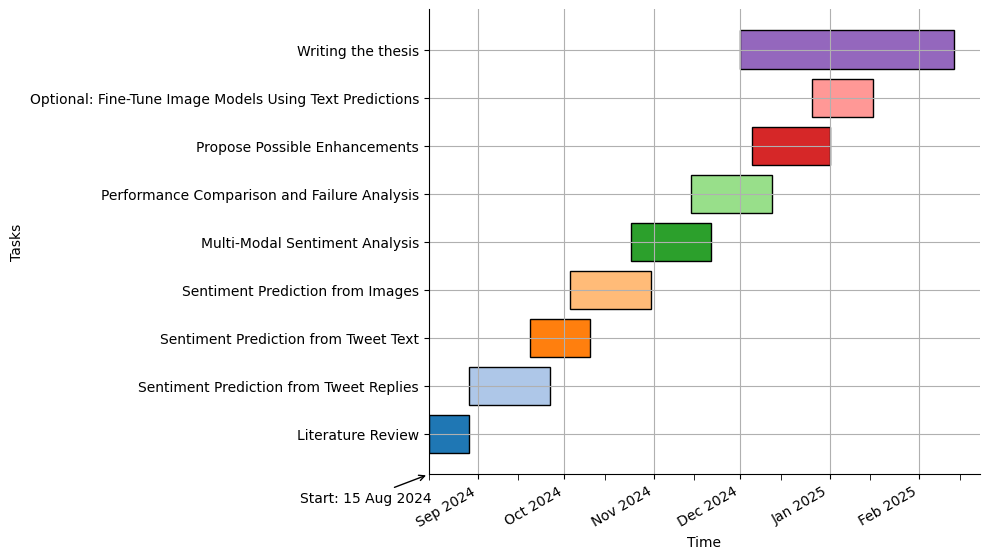
\includegraphics[width=\linewidth, height=0.3\textheight]{gantt}
    \caption{Gantt Chart for Thesis Timeline}
    \label{fig:gantt_chart}
\end{figure}

\newpage
\bibliographystyle{plain}
\bibliography{proposal}


\end{document}

